\subsection{Distributed Ledger Technology}

\subsubsection{Introduction to Distributed Ledger Technology}

Distributed ledger technology (DLT) is a recent invention which endeavours to make data publicly accessible through a decentralised system, providing no single point of failure. A DLT provides transparency where traditional centralised systems fall short and allows any willing and able party to be a part of the decentralised network. Furthermore, a DLT provides no easy way for any network moderator or specific party to control or override the network without the consensus of a significant number of the network's members. Combined, this technology introduces an entirely new way of dealing with transactional data and, as implemented below, any sort of data having a lifecycle.

\subsubsection{Blockchain}

The Blockchain~\footnote{\href{https://www.blockchain.com/}{Blockchain (https://www.blockchain.com)}} is the underlying technology that is used by cryptocurrencies such as Bitcoin~\footnote{\href{https://bitcoin.org/en/}{Bitcoin (https://bitcoin.org)}}. Since Blockchain was the first widely-available distributed ledger technology, most distributed ledger technologies since have chosen to adopt the blockchain name to refer to this architecture.

A traditional database is implemented such that it only maintains one current state for a given dataset~\footnote{Some databases have features allowing the user to view state (not transactions) over time (e.g. \href{https://www.postgresql.org/docs/6.3/static/c0503.htm}{PostgreSQL's Time Travel}) but these are not common and often deprecated} rather than transactions. In contrast, a blockchain, as the name would suggest, maintains a 'chain' of blocks of transactions that are agreed by the network forming a history of the chain's life. These blocks are formed of groups of transactions and are totally ordered across nodes in the network. It follows therefore that every node needs to have the entire history of the network, and that the provenance and origin of any given commodity, the unit of measure of a transaction, is maintained.

Whilst the above summarises the differences in the way a blockchain holds data compared to a traditional database, the differences in transaction ordering are far more fundamental and interesting. Consensus is used across a blockchain network to establish the most popular chain of transactions. It is possible for many chain possibilities to exist at any given time, but the longest chain is always assumed to be the main chain. Once a client has accepted a transaction (as part of a block), and it therefore forms part of their chain, it is not possible to choose another chain where this transaction has not been accepted (as part of the same block).

\subsubsection{Blockchain Consensus}

A few of the most popular methods of achieving consensus in a blockchain, and therefore total ordering, are listed below.

\begin{itemize}
  \item
    \textbf{Proof Of Work (PoW)}
    \textit{The majority of compute power in the network is held by honest members.~\footnote{Used by Bitcoin and Ethereum (pre-Serenity). \href{https://en.bitcoin.it/wiki/Proof_of_work}{Bitcoin Wiki}}}
  \item
    \textbf{Proof Of Stake (PoS)}
    \textit{The majority of stake (currency) in the network is held by honest members.~\footnote{Planned to be used by Ethereum (Serenity release and beyond). \href{https://www.cryptocompare.com/coins/guides/the-ethereum-releases-of-frontier-homestead-metropolis-and-serenity/}{Crypto Compare}}}
  % \item
  %   \paragraph{Byzantine Agreement (BA)}
  % \item
  %   \paragraph{Tendermint (TM)}
  % \item
  %   \paragraph{Stellar Consensus Protocol (SCP)}
\end{itemize}

\paragraph{Proof of Work}

Originally proposed as a method for countering denial of service attacks, Hashcash, authored by \cite{hashcash:1997:misc} and re-evaluated in \cite{hashcash:2002:online}, is the original proof of work scheme. The idea is that using cost-functions~\footnote{A cost-function should be parametrically expensive to compute, but efficiently verifiable. \cite{hashcash:2002:online}}, the hash of some $x$ is computed such that the left-most $n$ bits are equal to $0$. Since the hash of any two similar values is very different, as shown in program code \ref{code:example_keccak_unpredictability}, a cost-function designed in this way is difficult to compute.

\begin{listing}[H]
  \centering
  \begin{minted}{bash}
> hash('keccak256').update('Hello World!0').digest().toString('hex')
'2c6e6992915d52790a3625b459a0e7a1540a7770a6582f926d0119266b6f9f51'
> hash('keccak256').update('Hello World!1').digest().toString('hex')
'4d880de6488218d7153abeacff100608191ea63cccdd9894a602e8b3c959a276'
> hash('keccak256').update('Hello World!3').digest().toString('hex')
'f016006873889f59798ff191de74c0953892b38f77dbefc67b45af5ac705fcff'
  \end{minted}
  \caption{
    Variance between hashes of similar values
  }{
    Three similar values, shown to have very different hashes using the Keccak 256-bit hash function.
  }
  \label{code:example_keccak_unpredictability}
\end{listing}


As stated in the original Bitcoin paper (\cite{bitcoin:2008:misc}), the cryptocurrency uses Hashcash to provide block validation and to chain blocks of transactions together. As per Hashcash, the hash of the next (proposed) block must have the top $n$ bits set to zero. This value is how the network self-manages, adjusting $n$ according to a moving average of the number of blocks per hour. The hash of any particular block is computed by hashing the previous block's hash, the content of the block, and some nonce (a random value). As the nonce is incremented the hash of the block varies hugely and with sufficient iterations, the block will match the requirements of the next block.

Given the nonce we have a function difficult to compute but easy to verify, providing integrity to the underlying transactions, and ensuring that should any block be changed that's been verified, all child blocks (recursively) must be recomputed. If we assume that $51+\%$ of the compute power in the network is on honest nodes, then the longest chain will also be honest. Any malicious party would need to outpace the honest nodes in the network in order to take control and re-write the chain. The so-called $51\%$ attack is the most significant security threat to the proof-of-work model.

The proof-of-work model summarised above is used in the Bitcoin and Ethereum cryptocurrency systems for their main networks as of 15th June 2017.

\paragraph{Proof of Stake}

Intended as an alternative consensus mechanism to Proof of Work (PoW), Proof of Stake (PoS) uses a party's stake in the network to determine it's voting rights to the new block. This is in direct constrast to PoW which uses a party's compute power.

Neither Ethereum nor Bitcoin currently use proof of stake, although Ethereum is intending to use it in future releases. It remains a controversial consensus method, and as such is only summarised here.

As described by Ethereum~\footnote{\href{https://github.com/ethereum/wiki/wiki}{\textit{Ethereum Wiki}}}, there are two major consensus algorithms within the PoS category, \textbf{chain-based} and \textbf{Byzantine Fault Tolerance (BFT-style)}.

Within both of the major algorithms is the concept of a validator. A validator is someone who locks their ether as a deposit for a period of time. During this time, they are a current validator. In order to propose a block a party must be a current validator.

A chain-based algorithm uses a pseudo-random selection picking a current validator who is able to propose a block for a short time period. After this time period the validator changes. As in PoW the block proposed must point to some previously mined block, assuring a continuous chain is formed.

The BFT-style algorithm extends the idea behind the chain-based algorithm but over multiple rounds. In each round random validators are chosen to propose blocks. Over the rounds a consensus on a canonical block is reached, extending the chain.

% \paragraph{Byzantine}

% \paragraph{Stellar Consensus Protocol}

% \paragraph{Tendermint}

\subsubsection{Ethereum}

Ethereum extends the blockchain's uses beyond the direct exchange of currency and into the world whereby autonomous and publicly verifiable organisations and parties can live on the blockchain. By allowing the creation of so-called 'smart contracts', entities are established as part of the blockchain which can receive transactions from external parties (you and I). Through these transactions, the state of the contract is updated allowing the contract to function as a state transition system. Documentation and a Wiki page are the main sources of information on the Ethereum ecosystem~\footnote{\href{http://ethdocs.org/en/latest}{\textit{Read the Docs}, http://ethdocs.org/en/latest}}.

\paragraph{Ethereum Virtual Machine}

In the original blockchain, underpinning Bitcoin, a portion of every transaction is taken up by the script associated with performing it. In essence, this script represents the contract of the transaction. With Ethereum, the script transmitted with a transaction should be compatible with the Ethereum virtual machine (EVM). The EVM houses an environment where any conceivable computation of arbitrarily complexity can be achieved (turing-complete), with instructions authored and compiled in languages similar to JavaScript~\footnote{\href{https://solidity.readthedocs.io/en/develop/}{\textit{Solidity (Read the Docs)}, https://solidity.readthedocs.io/en/develop/}} and Python~\footnote{\href{https://github.com/ethereum/wiki/wiki/Serpent}{\textit{Serpent Wiki}, https://github.com/ethereum/wiki/wiki/Serpent}}. Through these languages contract code is compiled and 'activated' on an Ethereum network where it will be interacted with by externally-owned accounts (EOA). These interactions allow the realisation of the utility provided by the Ethereum network; the cryptographically secure underpinnings and distributed compute.

\paragraph{Decentralised Applications (DApps)}

With the EVM summarised above, we move to understanding the architecture of applications hosted by the Ethereum network and run on the EVM. A decentralised application (DApp) is an application whose's logic is hosted on the Ethereum network (through the medium of smart contracts) and interacting with the logic is done through a decentralised interface.

\subsubsection{Merkle Trees}

The importance of Merkle trees in the architecture and implementation of decentralised systems cannot be underestimated. When discussing the hashing of blocks above, the hash at the core of the block is that representing the integrity value of the transactions the block contains. As will be evidenced in the discussion of decentralised storage platforms, Merkle trees are at the very core of hashing the transactions in a block.

\cite{merkle:1988:inbook} authored a scheme to build trees where the content of a node could be validated as a function of the hash of other nodes. First one chooses a suitable hash function, and applies this to all leaf nodes in a possible tree. Then, one must apply the same hash function applied to the leaf nodes to the parent nodes such that every parent's hash is the hash of the sum of it's own value and the hashes of it's direct children. This structure results in a tree as in figure \ref{fig:example_merkle_tree}.

\begin{figure}[H]
  \centering
  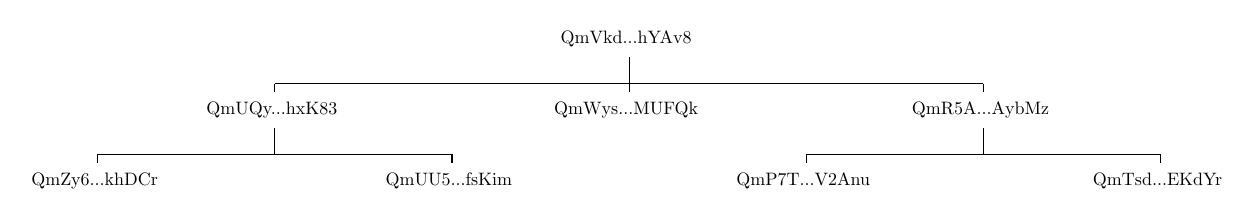
\begin{tikzpicture}[scale = 0.45, every node/.style={scale = 0.65}, every node/.append style={fill = white, rounded corners = 2pt, inner sep = 2pt, align = center}]

  \node at (0, 0) { QmVkd...hYAv8 };

  \draw (0, -0.5) -- (0, -1.5);
  \draw (-10, -1.25) -- (10, -1.25);
  \draw (-10, -1.25) -- (-10, -1.5);
  \draw (10, -1.25) -- (10, -1.5);

  \node at (-10, -2) { QmUQy...hxK83 };
  \node at (0, -2) { QmWys...MUFQk };
  \node at (10, -2) { QmR5A...AybMz };

  \draw (-10, -2.5) -- (-10, -3.25);
  \draw (-15, -3.25) -- (-5, -3.25);
  \draw (-15, -3.25) -- (-15, -3.5);
  \draw (-5, -3.25) -- (-5, -3.5);

  \draw (10, -2.5) -- (10, -3.25);
  \draw (15, -3.25) -- (5, -3.25);
  \draw (15, -3.25) -- (15, -3.5);
  \draw (5, -3.25) -- (5, -3.5);

  \node at (-15, -4) { QmZy6...khDCr };
  \node at (-5, -4) { QmUU5...fsKim };

  \node at (5, -4) { QmP7T...V2Anu };
  \node at (15, -4) { QmTsd...EKdYr };

  \end{tikzpicture}
  \caption{
    Example merkle tree
  }
  \label{fig:example_merkle_tree}
\end{figure}

